\documentclass[border=3pt,tikz]{standalone}
% Shared look for every TikZ figure in these notes.
% Included by each standalone figure file; also keeps the figures consistent
% with the colours used in the PDF and on the website.

\usepackage{tikz}
\usepackage{pgfplots}
\pgfplotsset{compat=1.18}
\usetikzlibrary{arrows.meta, decorations.markings, decorations.pathmorphing,
                patterns, calc, positioning}
\usepackage{amsmath}

% Series colours are the three validated categorical slots also used by the
% interactive widgets, so a path drawn in the printed notes and the same path on
% the website are the same colour. They clear the colour-vision-deficiency and
% contrast checks as a set; every path is direct-labelled as well, so colour is
% never the only thing carrying identity.
\definecolor{duPurple}{HTML}{68246D}
\definecolor{duBlue}{HTML}{2A78D6}
\definecolor{duRed}{HTML}{EB6834}
\definecolor{duGreen}{HTML}{1BAF7A}
\definecolor{duGrey}{HTML}{6B6B6B}

\tikzset{
  axisline/.style   = {-{Stealth[length=3mm]}, line width=0.7pt, black},
  path1/.style      = {duBlue,   line width=1.1pt},
  path2/.style      = {duRed,    line width=1.1pt},
  path3/.style      = {duGreen,  line width=1.1pt},
  statedot/.style   = {circle, fill=black, inner sep=1.4pt},
  arrowhead/.style  = {decoration={markings,
                        mark=at position #1 with {\arrow{Stealth[length=2.6mm]}}},
                       postaction={decorate}},
  lbl/.style        = {font=\small},
  slbl/.style       = {font=\footnotesize, duGrey},
  workfill/.style   = {duPurple, opacity=0.16},
}

% Kelvin scale: |Q|_rev is proportional to T; Q_C -> 0 at absolute zero
\begin{document}
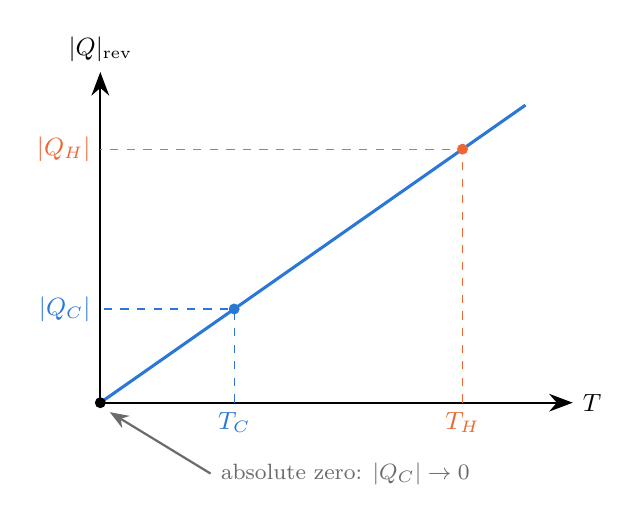
\begin{tikzpicture}[x=1cm,y=1cm]
  \draw[axisline] (0,0) -- (6,0) node[right, lbl] {$T$};
  \draw[axisline] (0,0) -- (0,4.2) node[above, lbl] {$|Q|_\text{rev}$};
  \draw[path1] (0,0) -- (5.4,3.78);
  \draw[duRed, dashed] (4.6,0) node[below, lbl] {$T_H$} -- (4.6,3.22) -- (0,3.22) node[left, lbl] {$|Q_H|$};
  \draw[duBlue, dashed] (1.7,0) node[below, lbl] {$T_C$} -- (1.7,1.19) -- (0,1.19) node[left, lbl] {$|Q_C|$};
  \node[statedot, fill=duRed] at (4.6,3.22) {};
  \node[statedot, fill=duBlue] at (1.7,1.19) {};
  \node[statedot] at (0,0) {};
  \draw[-{Stealth[length=2.4mm]}, duGrey, line width=0.8pt] (1.4,-0.9) node[right, slbl] {absolute zero: $|Q_C| \to 0$} -- (0.12,-0.12);
\end{tikzpicture}
\end{document}
